\documentclass[conference]{IEEEtran}
\IEEEoverridecommandlockouts
% The preceding line is only needed to identify funding in the first footnote. If that is unneeded, please comment it out.
%Template version as of 6/27/2024

\usepackage{cite}
\usepackage{amsmath,amssymb,amsfonts}
\usepackage{algorithmic}
\usepackage{graphicx}
\usepackage{textcomp}
\usepackage{xcolor}
\def\BibTeX{{\rm B\kern-.05em{\sc i\kern-.025em b}\kern-.08em
    T\kern-.1667em\lower.7ex\hbox{E}\kern-.125emX}}
\begin{document}

\title{Reconfigurable Energy Efficient Accelerator Architecture for CNN based Edge Applications
}

\author{
\IEEEauthorblockN{Muhammad Usman}
\IEEEauthorblockA{\textit{Centres of Excellence in Science \&} \\
\textit{Applied Technologies (CESAT)} \\
\textit{Islamabad, Pakistan} \\
i201320@nu.edu.pk}
\and
\IEEEauthorblockN{Azhar Zahid}
\IEEEauthorblockA{\textit{Centres of Excellence in Science \&} \\
\textit{Applied Technologies (CESAT)} \\
\textit{Islamabad, Pakistan} \\
i201312@nu.edu.pk}
\and
\IEEEauthorblockN{Abdul Moiz Sheikh}
\IEEEauthorblockA{\textit{Centres of Excellence in Science \&} \\
\textit{Applied Technologies (CESAT)} \\
\textit{Islamabad, Pakistan} \\
}
}
\maketitle
\begin{abstract}
Real-time artificial intelligence (AI) applications demand significant computational resources, often exceeding the capabilities of general-purpose processors. Consequently, research focus has shifted towards application-specific hardware, known as AI accelerators. This work presents an optimized AI accelerator architecture emphasizing memory hierarchy design to enhance performance and energy efficiency. Since memory access contributes substantially to overall delay and power consumption, the proposed architecture integrates multi-level memory for efficient data reuse and minimize redundant data transfers. Additionally, a tiling-based processing approach is employed to perform convolution, pooling, activation, and batch normalization operations in parallel across individual tiles, thereby reducing hardware resource utilization. To demonstrate scalability beyond simple convolutional models, the architecture is evaluated on representative modern vision workloads, including ResNet for residual image classification and Tiny-YOLO for real-time edge object detection. The proposed design achieves a peak throughput of 90~GOPS with a power consumption of 218~mW after synthesis on the open-source SkyWater 130~nm ASIC technology, corresponding to an energy efficiency of 412.84~GOPS/W at 100~MHz. The results demonstrate a 65\% improvement in power efficiency compared to state-of-the-art implementations, validating the effectiveness of the proposed memory-optimized accelerator architecture.
\end{abstract}

\begin{IEEEkeywords}
Edge AI, Hardware Accelerator, Convolutional Neural Networks, Memory Hierarchy, ResNet, Tiny-YOLO, SkyWater 130 nm.
\end{IEEEkeywords}

\section{Introduction}
\label{sec:intro}
Convolutional Neural Networks (CNNs) are among the most widely used architectures in deep learning, particularly suited for processing two-dimensional data through their convolutional layers \cite{CIACON2025_Optimizing_CNN}. From a computational perspective, the convolution operation dominates the workload, involving intensive multiply–accumulate (MAC) operations between input feature maps and kernel weights. These operations require a substantial number of multipliers and adders, as well as frequent memory accesses, leading to significant latency and power consumption \cite{ISCAS2025_Weight_Approximation_and_Data_Reuse}.

Conventional CPUs lack the parallel computing capability required for such workloads, while GPUs, though offering improved parallelism, suffer from high power consumption and limited power efficiency for real-time AI applications \cite{ICCSP2025_Edge_AI}. Consequently, there is a growing demand for dedicated and energy-efficient hardware accelerators capable of supporting diverse AI workloads. Google’s Tensor Processing Unit (TPU) represents one such advancement; however, still AI accelerator design remains an active and evolving research area.

Various optimization techniques have been proposed to enhance accelerator performance, including systolic arrays, memory reuse, loop unrolling, and approximate multipliers. The fundamental computational block in most of these designs is the Processing Element (PE) \cite{Usman2025}, which performs the MAC operations utilized in CNN processing. Additionally, caching and data reuse are also critical for reducing off-chip memory communication and improving throughput \cite{ISCAS2025_Weight_Approximation_and_Data_Reuse}.

The motivation behind this research is to develop a custom hardware architecture that efficiently executes AI workloads. The proposed accelerator focuses on two primary features:
\begin{enumerate}
    \item Reconfigurable Processing Elements (PEs) and fused processing cores for flexible operation mapping across diverse neural workloads, including residual networks (e.g., ResNet) and multi-scale object detection models (e.g., Tiny-YOLO).  
    \item Hierarchical caching and row-buffered data reuse mechanisms to minimize external memory access.  
\end{enumerate}
This design aims to achieve high computational efficiency and energy savings, addressing the challenges in deploying AI models on resource-constrained platforms.

\section{State-of-the-Art Literature Review}
\label{sec:literature}

Several hardware platforms like GPUs, TPUs, FPGAs and ASICs are utilized to accelerate AI workloads, each optimized for specific performance, flexibility, and power trade-offs.
% \begin{enumerate}
%     \item Graphics Processing Units (GPUs) are widely used for parallel processing in deep learning and computer vision applications.
%     \item Tensor Processing Units (TPUs) are purpose-built for deep learning workloads, offering high throughput and efficiency.
%     \item Field-Programmable Gate Arrays (FPGAs) provide reconfigurability for customized AI inference.
%     \item Application-Specific Integrated Circuits (ASICs) deliver maximum performance and energy efficiency for fixed workloads.
% \end{enumerate}
These platforms are deployed in edge devices, data centers, and embedded systems for applications such as image recognition, natural language processing, and autonomous systems. Few recent hardware accelerators are discussed below:

\subsection{Three-Dimensional GEMM Architecture with RISC-V~\cite{16TOPS_GEMM}}
An efficient General Matrix Multiplication (GEMM) module was proposed as the core of a Deep Learning Accelerator (DLA), integrating a RISC-V processor for scalar control and a processing engine for tensor operations as shown in Fig. \ref{GEMM}. The GEMM module features 4096 MAC units supporting FP16 and INT8 computations with resource reuse through pipelined execution. The architecture employs a three-dimensional MAC arrangement for fine-grained control and high scalability via a hierarchical instruction queue. However, varying workload sizes may cause underutilization of resources, leading to the dark silicon effect.
\begin{figure}[t]
\centering
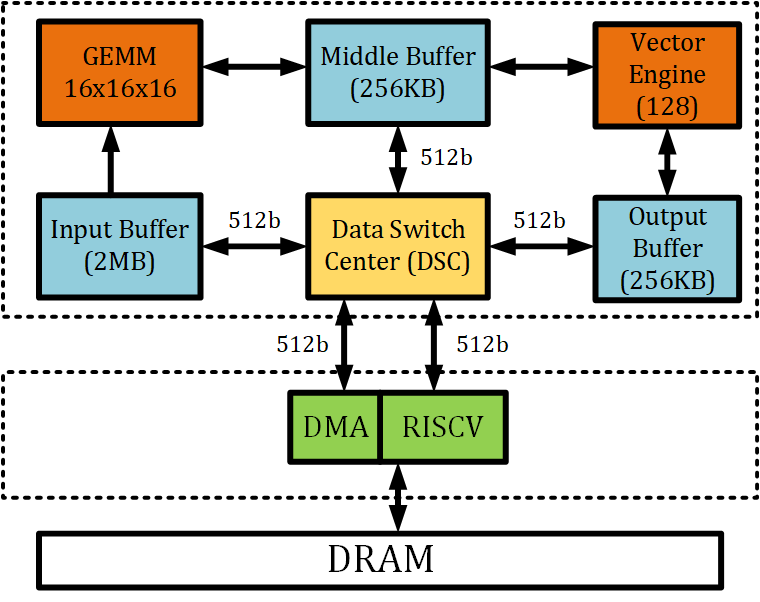
\includegraphics[width=1.0\columnwidth,keepaspectratio]{pictures/GEMM.jpg}
\caption{Top Level architecture for DLA based on GEMM\cite{16TOPS_GEMM}}
\label{GEMM}
\end{figure}
\subsection{Memory-Centric Modular Architecture for Neural Networks~\cite{mem_centric_NPU}}
A modular Neural Processing Unit (NPU) architecture was introduced, consisting of 16 Processing Elements (PEs) and a local SRAM to enable configurable parallelism and data reuse with architecture shown in Fig. \ref{mem_centric}. The design supports multiple convolution modes—depth-wise, point-wise, and 2D—through SRAM-based data configuration. By placing memory near the PEs, the design minimizes latency and power consumption. However, the fixed number of PEs may result in inefficiency for workloads that do not align with the hardware configuration.
\begin{figure}[t]
\centering
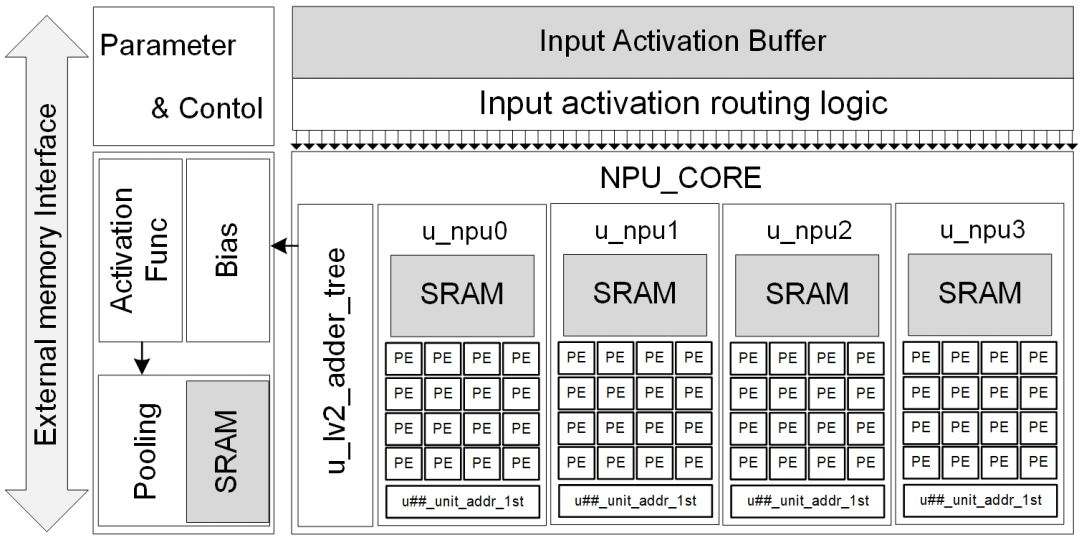
\includegraphics[width=1.0\columnwidth,keepaspectratio]{pictures/mem_centric.JPG}
\caption{Hardware configuration of Neural Engine for VGG-16\cite{mem_centric_NPU}}
\label{mem_centric}
\end{figure}
\subsection{Low-Power Architecture Exploiting Memory Hierarchy Optimization~\cite{eyeresis_v2}}
The row-stationary (RS) dataflow was proposed to reduce data movement energy cost in spatial architectures. This approach maximizes local data reuse of filter weights, activations, and partial sums across four storage hierarchy levels: DRAM, global buffer, inter-PE communication, and local register files. The design employs direct inter-PE communication and spatial parallelism to minimize high-cost DRAM accesses, significantly improving energy efficiency for CNN workloads.

\subsection{Low-Power Architecture for Extreme Edge Inference~\cite{TinyVers}}
TinyVers’ FlexML accelerator targets ultra-low-power \textit{tinyML} applications. It features an 8$\times$8 SIMD array of precision-scalable MAC-based PEs, supporting runtime reconfigurable dataflow with zero-latency switching as shown in Fig. \ref{TinyVers_image}. The architecture enables symmetric precision quantization for activations and weights, minimizing hardware overhead while maximizing data reuse. Output normalization through simple shift and ReLU operations further reduces computational cost. Although the design efficiently supports diverse ML workloads, mixed-precision handling may introduce bandwidth and control challenges.
\begin{figure}[t]
\centering
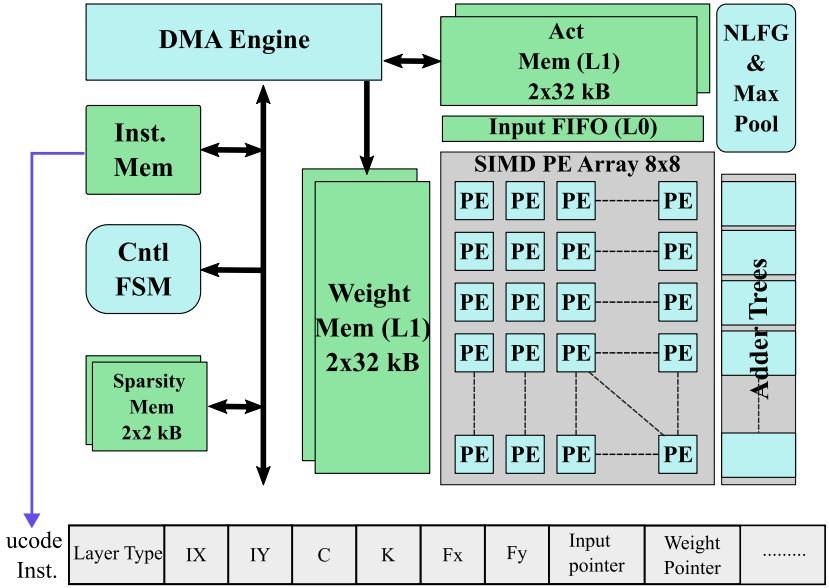
\includegraphics[width=1.0\columnwidth,keepaspectratio]{pictures/TinyVers.JPG}
\caption{Top Level architecture for DLA based on GEMM\cite{TinyVers}}
\label{TinyVers_image}
\end{figure}

\section{Proposed Methodology}
\label{sec:methodology}
The hierarchy of proposed architecture begins with a “Processing Element (PE)”, and then comes the “Engine”, followed by a “Core” and then a ”Mega Core” with it is a “Top Memory” and lastly the complete “Accelerator”. The bit precision(bp) of the accelerator is selected to be INT8 fixed for both weights and Input/Output feature values. The size of the input feature matrix is taken as 32x32, while for weights it is 3x3. As a proof of concept the architecture is designed to implement Le-Net5 Neural Network. The detailed explanation of sub blocks is given below:

\subsection{Processing Element (PE)}
The PE is basic workhorse in convolution operation and is responsible for the multiplication of feature and weight values. The inputs to PE are clock, enable, reset and weight value as shown in \ref{processing_element}. However, the PE is unique in terms of its input feature. The PE has three inputs $IF_{in1}$, $IF_{in2}$, $IF_{in3}$ for input feature instead of one. $IF_{in1}$ is the input used immediately by the weight, $IF_{in2}$ is used in 2nd iteration and $IF_{in3}$ is used in third iteration of the weight feature multiplication. The value to be used in particular iteration depends on the value of “control” signal, which is also a 2-bit input to the PE. The PEs overall hardware consists of a Multiplier, a Mux and a register for storing the value at the particular iteration. The PE takes the the input with INT8 bit precision (bp) yielding the output value with INT16 bit precision, while taking three cycles to give output for one value of the input feature.

\begin{figure}[t]
\centering
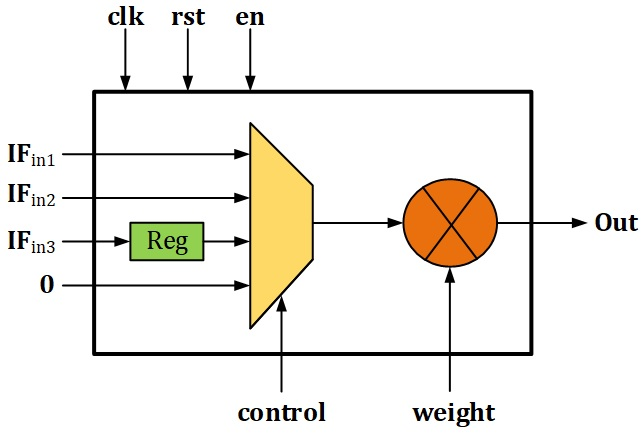
\includegraphics[width=1.0\columnwidth,keepaspectratio]{pictures/pe.jpg}
\caption{Processing Element}
\label{processing_element}
\end{figure}

\subsection{The Processing Engine}
The next level in the hierarchy is the engine, with each engine consisting of two sets of 9 PEs as shown in \ref{processing_engine}. Each PE is connected to one of the 9 weights. The system assumes a weight stationary workload and the weights can only be changed when the engine is in “reset” or “not enable mode”.  Each set of 9 PEs has an adder tree which adds the outputs of the PEs together. Each engine is responsible for the convolution of a weight matrix with size(kh,kw)=3x3  and input feature matrix with size(Hs,Ws)=8x8. The engine has one feature buffer which is capable of storing 3 rows of (Hs,Ws) feature matrix. When the engine has its first three rows the operation starts. The engine is capable of producing the first row of 6x6 resulting matrix in 4 cycles. The engine also features an FSM-based control unit that generates the control input and dictates the operation of PEs and the engine. When the value of control is “0” the engine is allowed to take the value of next row of 8x8 input feature matrixes. On value “1” the PE units multiply the input $IF_{in1}$ to the weight value. On value “2” the value at $IF_{in2}$ is multiplied and on “3” the value at $IF_{in3}$ is used. The connections to the three inputs for features are done via the input buffer with each input connected to its respective bit addressed value in buffer. The two sets of 9 PEs generate outputs in parallel.  
\begin{figure}[t]
\centering
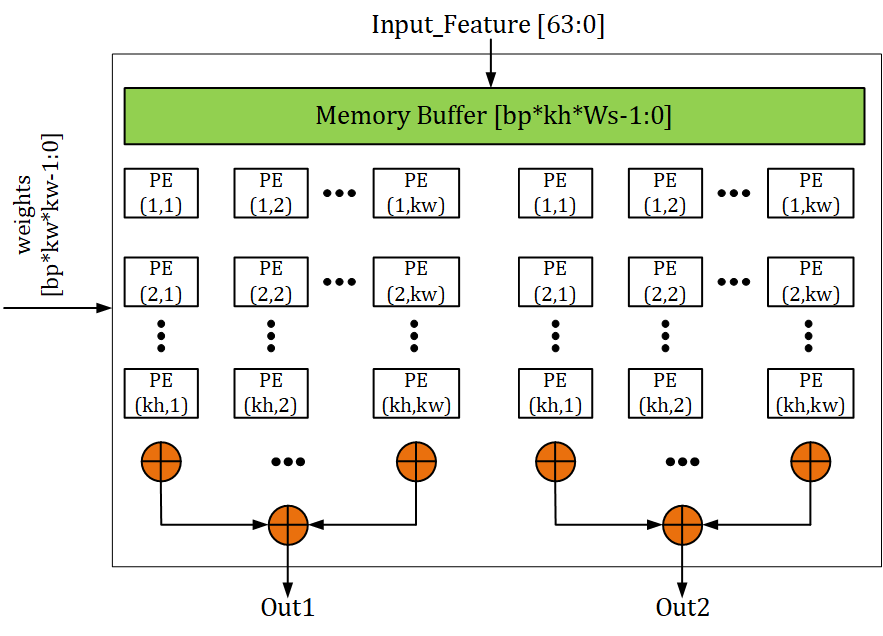
\includegraphics[width=1.0\columnwidth,keepaspectratio]{pictures/engine.jpg}
\caption{Proposed Processing Engine}
\label{processing_engine}
\end{figure}
% The engine architecture is such that it facilitates the use of 1D operations, if the operations can be zero padded or parallelized for multiple vectors. The zero padding case can be implemented but would require a specific pattern of zero padded values for proper operation.
% The value of state variable generated in the engine also acts as a control signal in the other units such as buffer and enabling of Max-pooling unit as well as for top core sram controller.
\subsection{The Processing Core}
The level above the engine is the core. The core consists of one “Register file” with 64x8 bit dimensions. The register file is dual-port to allow pipelining between receiving data from the outside and feeding it to engine underneath. The Register file is chosen due to its lower area and better performance characteristics as compared to SRAM. The size of Register file is such that it is capable of holding an 8x8 feature matrix with a INT8 bit precision (bp). The addresses of the Reg file are generated by a small controller which is built with the register file. This controller provides a distributed control for each respective SRAM. This also produces addresses in fixed pattern since the engine processes the features in a fixed flow and not much flexibility is needed at this level for address generation.   
The component next to the Register file is the Engine (as described in previous subsection, which is fed the feature data from the Register file. The operation of the engine is enabled as soon as the Register file is fed the first three rows of feature 8x8 matrix. when the engine is ready for the next feature data it gives the feedback to the controller of register file, and the next value is fed to the engine from the register file. This allows pipelining between feeding data and processing it. 
% Also it can be noted that the engine performing convolution does not do zero padding to feature vector.
The next unit in the core is the output “Buffer”. The buffer is capable of holding 6x2 values of the output of engine i.e. two rows of the 6x6 output of the convolution results with INT16 precision. This buffer acts as input to the max-pooling, activation or batch normalization unit. Once the buffer is full, the maxpooling, activation or batch normalization unit is enabled to perform the relevant operation.
Overall the core takes an 8x8 sub-section of the 32x32 input feature map along with the 3x3 weight vector. The result coming out of the core is a 3x3 max-pooled output in case of LeNet-5. This fusion of the convolution and pooling step allows for lesser hardware and lesser latency since applying pooling on a smaller matrix can be parallelized without the need for adding too much hardware. Since the pooling is parallelized on the 6x2 value buffer, the output is generated in one cycle and there is no need to iterate a large matrix as would be the case of traditional maxpooling on the complete 30x30 output of a traditional Le-Net 1st layer convolution. The overall architecture of the core is shown below in Fig. \ref{processing_core}.
\begin{figure}[t]
\centering
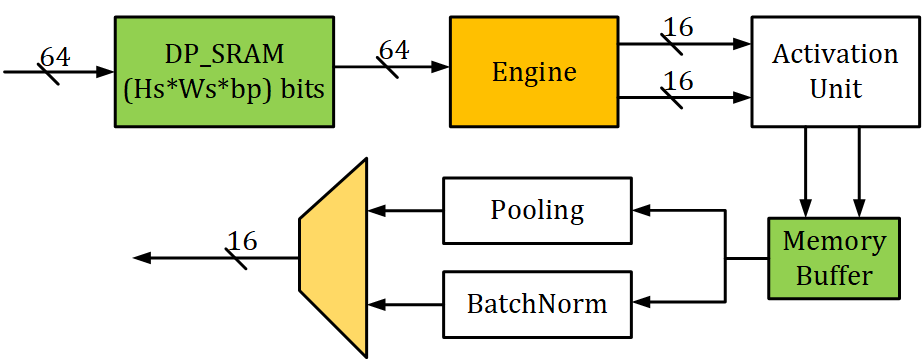
\includegraphics[width=1.0\columnwidth,keepaspectratio]{pictures/core.jpg}
\caption{Proposed Processing Core}
\label{processing_core}
\end{figure}
\subsection{The Mega Core(Overall Accelerator)}
The mega core takes a 256 bit vector as an input i.e. a 32x1 vector with an INT8 precision. This is provided by the SRAM on top of the mega core. This 256 bit vector is used to fill up the internal register files of the cores. The mega core also takes a 3x3 weight matrix with an INT8 precision as input. This is in fact a 72 bit vector with 9 values and each as 8 bits. The mega core also has a control mechanism implemented as a simple state machine counter combination to determine which core is filled up with the incoming input of 256 bit feature vector. The mega core has 5 buffers which store outputs of the results of the cores and give them at the output. Each buffer is 240 bits long i.e. can store 15 values with INT16 precision. This is effectively one row of the output 15x15 matrix with INT16 precision.
The mega core consists of 25 cores each with its own register file, control unit for register file, convolution engine, buffer and maxpooling, activation and batch normalization unit. Each mega core is divided into five rows of five cores. Each row has a buffer which is capable of storing a 255 bit value. The segregation is done such that the effective stride of convolution matrix is one i.e., the last two values of the core1 are first two values of core2 in row 1 of the mega core. The cores within the mega core are all assigned the same weight 3x3 matrices. This ensures the weight stationary behavior and hence achieves parallelism in computing the results. 
The output of the mega core are the five buffers from each row of the core. The output is the vector of dimension  240(15x16)x1. Each row produces results at one cycle and no two rows produce results simultaneously. This is due to the fact that the data input to the mega core is one row at a time and the individual rows get filled in a round robin fashion and not continuously. This delay in output enables the result to be added to the results of the other kernels and stored to the output SRAM. Each buffer changes value three times for each 32x32x1 input. This results in a 15x15 matrix output. This output is stored in the output sram and can be transferred outside the chip.
\begin{figure}[t]
\centering
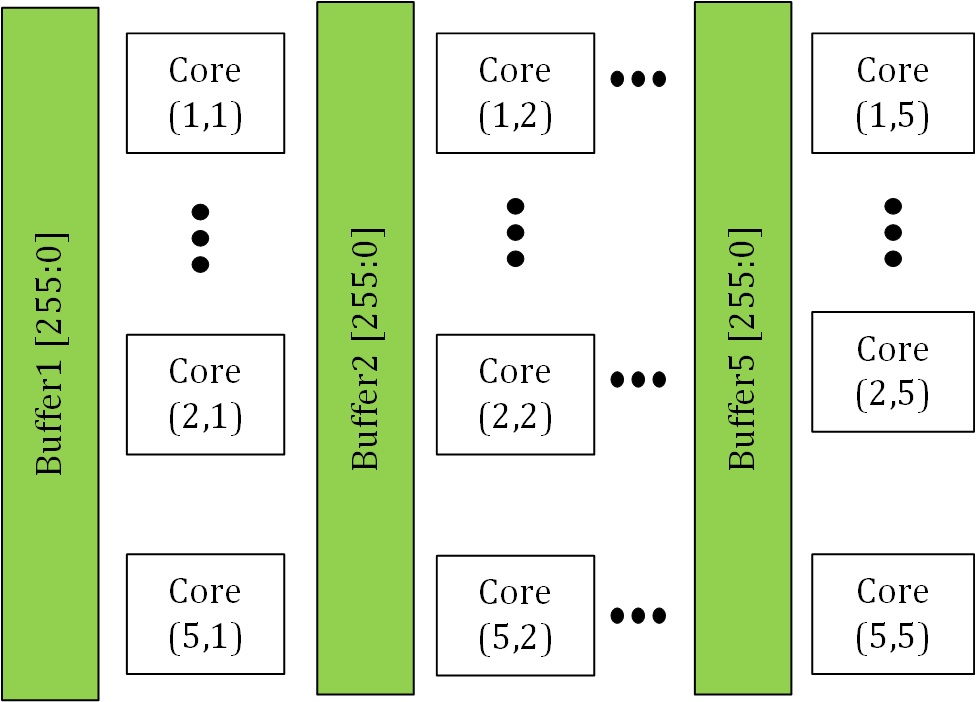
\includegraphics[width=1.0\columnwidth,keepaspectratio]{pictures/accelerator.jpg}
\caption{Proposed Accelerator (The Mega Core)}
\label{accelerator}
\end{figure}
\subsection{Workload Mapping: ResNet and Tiny-YOLO}
To evaluate the flexibility and scalability of the proposed accelerator beyond proof-of-concept topologies, execution flows for modern deep learning models—specifically deep residual networks (ResNet-18/20) and real-time detection architectures (Tiny-YOLOv2/v3)—are mapped onto the hardware:

\subsubsection{ResNet Mapping}
Deep residual models rely heavily on repetitive $3\times 3$ convolutional layers alternating with $1\times 1$ pointwise projection layers and residual skip additions ($F(x) + x$). In our architecture, standard $3\times 3$ convolutions are mapped across the 25 processing cores by partitioning input feature maps across the channel dimension into $8\times 8$ spatial tiles accommodated inside the local dual-port register files. PEs operate in weight-stationary mode across spatial activations. For $1\times 1$ projection shortcuts, the PE control logic dynamically disables two taps, utilizing single-tap multiplier execution with direct register forwarding to sustain computational throughput. Crucially, residual skip additions are executed directly during the write-back phase into the top dual-port output SRAM prior to the activation stage. This on-chip accumulation completely eliminates the need to spill intermediate residual feature maps to external memory.

\subsubsection{Tiny-YOLO Mapping}
Tiny-YOLO object detectors process high-resolution input frames (e.g., $224\times 224$ or $416\times 416$) through consecutive convolution and downsampling stages to predict multi-scale bounding boxes. To accommodate larger spatial dimensions, input images are streamed through the 5-row buffer using a round-robin tile loading schedule. Successive convolutional stages are pipelined with the integrated pooling units, which perform $2\times 2$ max-pooling with stride 2 directly on the $6\times 2$ output buffers within a single clock cycle, effectively fusing convolution and pooling operations without intermediate DRAM traffic. Furthermore, the core activation unit supports the piecewise-linear Leaky ReLU ($\alpha = 0.1$) non-linear activation function required by the Darknet backbone before writing final detection tensors to the output memory.

\section{Results and Discussions}
\label{sec:results}
The design was synthesized using Sky130nm technology which is a legacy node but the Process Design Kit (PDK) is open source. The whole process was carried out using open source toolchains Yosys, Openlane and OpenRAM. The clock frequency for the said design was 100MHz. The memory modules were placed as hard macros in the design and their characterization was done at Typical (TT) process corner.

\subsection{Hardware Synthesis and ASIC Comparison}
A comprehensive comparison of the proposed accelerator with state-of-the-art designs implemented on the SkyWater 130~nm node and related edge platforms is summarized in Table~\ref{tab:comparison}. Operating at 100~MHz with INT8 precision, the proposed design achieves a peak throughput of 90~GOPS and an energy efficiency of 412.844~GOPS/W. Compared to the open-source inference engine in MWSCAS'21~\cite{Nasser2021} (19.2~GOPS, 246.15~GOPS/W), our architecture achieves a $4.68\times$ throughput speedup and a $67.7\%$ efficiency improvement owing to local register-file tiling and data reuse across the 25 processing cores. 

Furthermore, compared to the shared-unit CNN accelerator in MWSCAS'24~\cite{Khalil2024} (28.41~GOPS/W at 120~MHz) and the 2D-mesh NoC systolic accelerator in Appl. Sci.'26~\cite{Mascorro2026} (38.10~GOPS/W, 378~mW at 100~MHz), the proposed design achieves $14.5\times$ and $10.8\times$ higher energy efficiency, respectively, while consuming lower total power than the NoC-based approach. This stems from our deterministic row-buffered streaming, which eliminates heavy NoC packet routing and dynamic switching overheads. Finally, compared to the JSSC'23 TinyVers SoC~\cite{TinyVers} (250~GOPS/W, 11.7~GOPS), our accelerator yields a $7.69\times$ throughput boost and a $65\%$ higher GOPS/W, validating that dense parallel core scaling significantly enhances edge throughput without compromising energy efficiency.

\begin{table}[t]
\centering
\caption{Comparison with State-of-the-Art Silicon Implementations}
\label{tab:comparison}
\footnotesize
\setlength{\tabcolsep}{2.2pt}
\begin{tabular}{@{}lccccc@{}}
\hline
\textbf{Parameter} & \textbf{MWSCAS} & \textbf{MWSCAS} & \textbf{Appl. Sci.} & \textbf{JSSC} & \textbf{This} \\
 & \textbf{'21 \cite{Nasser2021}} & \textbf{'24 \cite{Khalil2024}} & \textbf{'26 \cite{Mascorro2026}} & \textbf{'23 \cite{TinyVers}} & \textbf{Work} \\
\hline
Technology        & Sky130 & Sky130 & Sky130 & Sky130 & Sky130 \\
Freq. (MHz)       & 100    & 120    & 100    & 100    & 100   \\
Precision         & INT8   & INT8   & Fixed  & INT8   & INT8  \\
Peak GOPS         & 19.2   & 3.3    & 14.4   & 11.7   & 90    \\
Power (mW)        & 78     & 115    & 378    & 46.8   & 218   \\
GOPS/W            & 246.15 & 28.41  & 38.10  & 250    & 412.84 \\
\hline
\end{tabular}
\end{table}

\subsection{Workload Evaluation and Comparison for ResNet and Tiny-YOLO}
To evaluate end-to-end performance on practical edge workloads, the mapped ResNet and Tiny-YOLO network models are compared against published state-of-the-art accelerators in Table~\ref{tab:model_comparison}.

For image classification using residual networks, representative implementations include SPARX'24~\cite{sparx2024} (an approximate FPGA accelerator achieving 800~FPS on ResNet-20 at 2.1~W), Liu \textit{et al.}'23~\cite{liu2023tvlsi} (a 65~nm reconfigurable ASIC achieving 127.8~FPS and 7.82~ms latency on ResNet-18 consuming 42.6~mW), and the multi-mode TinyVers SoC~\cite{TinyVers} on SkyWater 130~nm (38.2~FPS at 20.4~mW). The proposed 25-core architecture leverages parallel weight-stationary execution and local dual-port register file tiling to minimize memory bottlenecks during channel-dense convolutions.

For real-time object detection using Tiny-YOLO models, recent benchmarks include the FPGA TPU design in Rossi \textit{et al.}'25~\cite{yolov3tiny2025} (208.3~FPS on YOLOv3-Tiny consuming 2.55~W on a Zynq-7020), the lightweight Zynq-7000 accelerator by Nguyen \textit{et al.}'20~\cite{nguyen2020tcas} (44.6~FPS on Tiny-YOLOv2 at 1.98~W), and the 28~nm ASIC implementation YOLO-Edge'24~\cite{yoloedge2024} (195.3~FPS at 58.0~mW). By fusing the convolution and max-pooling pipelines directly in each core and buffering feature rows through the dedicated Mega Core buffers, our architecture is structured to sustain high-throughput inference without off-chip memory penalties.

\begin{table*}[t]
\centering
\caption{Performance Comparison for ResNet and Tiny-YOLO Workloads}
\label{tab:model_comparison}
\footnotesize
\setlength{\tabcolsep}{8pt}
\begin{tabular}{@{}llccccc@{}}
\hline
\textbf{Model} & \textbf{Work} & \textbf{Platform} & \textbf{Frequency (MHz)} & \textbf{Latency (ms)} & \textbf{Throughput (FPS)} & \textbf{Power} \\
\hline
\multicolumn{7}{l}{\textit{\textbf{ResNet Benchmark (ResNet-18 / ResNet-20)}}} \\
\hline
ResNet-20 & SPARX'24 \cite{sparx2024}     & VC707 FPGA   & 200 & 1.25 & 800.0 & 2.1 W \\
ResNet-18 & Liu \textit{et al.}'23 \cite{liu2023tvlsi} & 65\,nm ASIC  & 200 & 7.82 & 127.8 & 42.6 mW \\
ResNet-18 & TinyVers'23 \cite{TinyVers}   & Sky130 ASIC  & 100 & --   & 38.2  & 20.4 mW \\
ResNet    & \textbf{This Work}            & \textbf{Sky130 ASIC} & \textbf{100} & \textbf{--} & \textbf{--} & \textbf{--} \\
\hline
\multicolumn{7}{l}{\textit{\textbf{Tiny-YOLO Benchmark (v2 / v3 / v4)}}} \\
\hline
YOLOv3-T  & Rossi \textit{et al.}'25 \cite{yolov3tiny2025} & Zynq-7020 FPGA & 200 & 4.80 & 208.3 & 2.55 W \\
YOLOv2-T  & Nguyen \textit{et al.}'20 \cite{nguyen2020tcas} & Zynq-7000 FPGA & 150 & 22.4 & 44.6  & 1.98 W \\
YOLO-Tiny & YOLO-Edge'24 \cite{yoloedge2024} & 28\,nm ASIC & 250 & 5.12 & 195.3 & 58.0 mW \\
Tiny-YOLO & \textbf{This Work}            & \textbf{Sky130 ASIC} & \textbf{100} & \textbf{--} & \textbf{--} & \textbf{--} \\
\hline
\end{tabular}
\end{table*}

\section{Conclusion}
\label{sec:conclusion}
The proposed work presents an energy-efficient hardware architecture optimized for accelerating diverse deep learning workloads at the extreme edge. By integrating a multi-level memory hierarchy with local register-file tiling, fused convolution-pooling cores, and weight-stationary processing engines, the design effectively mitigates memory access latency and power consumption. The accelerator demonstrates scalable mapping for both deep residual networks (ResNet) and real-time detection architectures (Tiny-YOLO). Synthesized on the open-source SkyWater 130~nm ASIC node, the design achieves a peak throughput of 90~GOPS with a power consumption of 218~mW at 100~MHz, corresponding to an energy efficiency of 412.84~GOPS/W and outperforming comparable state-of-the-art designs by up to 65\%. Future work includes extending the control fabric for variable-precision arithmetic to further optimize latency and efficiency across diverse edge AI domains.
\bibliographystyle{IEEEtran}
\bibliography{refer}


\end{document}
